\documentclass[conference]{IEEEtran}
\IEEEoverridecommandlockouts

\usepackage{cite}
\usepackage{amsmath,amssymb,amsfonts}
\usepackage{graphicx}
\usepackage{booktabs}
\usepackage{array}
\usepackage{textcomp}
\usepackage{xcolor}
\usepackage{url}
\usepackage{float}
\usepackage{tikz}
\usepackage[colorlinks=true,linkcolor=black,urlcolor=blue,citecolor=black]{hyperref}
\usetikzlibrary{positioning,arrows.meta}


\hypersetup{
    pdftitle={Data Engineering II Mini Project --- Group 16},
    pdfauthor={Group 16, Uppsala University}
}

\def\BibTeX{{\rm B\kern-.05em{\sc i\kern-.025em b}\kern-.08em
    T\kern-.1667em\lower.7ex\hbox{E}\kern-.125emX}}

\begin{document}

\title{A Scalable GitHub Analytics System Using Apache Pulsar}

\author{
\IEEEauthorblockN{
    Tejas Chakravarthy,
    Andreas Hadjoullis,
    Julios Fotiou,
    Tanay Singh,
    Adnan Erlangga Raharaja
}
\IEEEauthorblockA{
    Uppsala University \\
    1TD076 Data Engineering II, VT 2026, Group 16 \\
    Source code: \url{https://github.com/tj-chakravarthy/Data-Engineering-II-Project-2}
}
}

\maketitle

\begin{abstract}
% Write this last.
% Briefly describe:
% 1. the problem,
% 2. the proposed system,
% 3. the main technologies,
% 4. the experiments,
% 5. the main findings.

\end{abstract}

\begin{IEEEkeywords}
GitHub API, Apache Pulsar, stream processing, container orchestration, data analytics
\end{IEEEkeywords}

\section{Introduction}
GitHub hosts a large number of open-source software projects and provides
repository metadata through its REST API~\cite{github_rest_api}. This metadata can be useful for
understanding software development trends, such as which programming languages
are most common, which repositories are actively maintained, and how often
projects use unit tests and continuous integration. However, these higher-level
analytics are not directly available through GitHub search. Therefore, a data
engineering pipeline is needed to collect, process, and analyze repository
metadata at scale.

This project develops a GitHub analytics system using Apache Pulsar as the
streaming framework~\cite{apache_pulsar}. The system collects repository metadata from the GitHub
API, publishes it to Pulsar topics, and processes it using worker services to
produce the required analytics. The analytics component is designed to answer
the project questions, including the most common programming languages, the
most frequently updated repositories, the languages most associated with unit
testing, and the languages most associated with both unit testing and
continuous integration.
The system also addresses practical data engineering challenges. GitHub search
results are limited, so the crawler must divide the collection process into
smaller queries and use pagination. API rate limits must also be considered
when collecting repository metadata. To make the system reproducible and easier
to deploy, the implementation uses Docker containers and automation scripts.
The main contribution of this work is the design of a cloud-based and scalable
GitHub analytics pipeline using suitable data engineering frameworks. Apache
Pulsar is used as the streaming layer, while containerization and automation
support deployment across multiple virtual machines.

\section{Related Work}
\label{sec:related-work}
GitHub is widely used as a data source in empirical software engineering and
mining software repository research. Kalliamvakou et al. show that GitHub
metadata can provide useful information about software development activity, but
also emphasize that such data must be interpreted
carefully~\cite{kalliamvakou2014promises}. This is relevant to the present
project because repository metadata is used to derive analytics about
programming languages, update activity, unit testing, and continuous
integration.

Stream processing systems are useful when data should be processed
incrementally rather than only after a complete dataset has been collected.
Blamey et al. compare stream-processing systems using throughput-oriented
benchmarks under different processing loads~\cite{blamey2019apache}. In this
project, Apache Pulsar is used as the streaming layer, following a
producer-topic-consumer model where repository records are published as
messages and processed by worker services~\cite{apache_pulsar}.

Cloud deployment and automation are also relevant because the system is
intended to run across multiple virtual machines. Armstrong et al. discuss
cloud contextualization as a way to configure virtual machines during
deployment~\cite{armstrong2015contextualization}. In this project,
containerization and automation are used to make the pipeline more reproducible
and easier to deploy across cloud resources.


\section{System Architecture}
\label{sec:architecture}

\subsection{Overview}
The proposed system is designed as a cloud-based streaming pipeline for
collecting, enriching, and analyzing GitHub repository data.
Figure~\ref{fig:architecture} shows the high-level architecture of the system.
The architecture separates the pipeline into three main stages: data collection,
repository metadata enrichment, and data aggregation. This separation allows the
runners responsible for enriching the metadata repository to be developed,
deployed, and scaled independently.

The pipeline starts with a crawler that retrieves repository metadata from the
GitHub API. Each repository is converted into a structured record and published
to a raw repository stream. A configurable number of processing runners consume
these records and enrich them with additional information using the GitHub API.
This enrichment is necessary because the initial metadata is not sufficient to
answer all project questions, especially those related to commit activity,
unit-test usage, and CI/CD usage. The runners then publish data to an
aggregation stream. Finally, the aggregator computes a new answer to each
question based on all aggregated data so far.

\begin{figure}[!t]
\centering
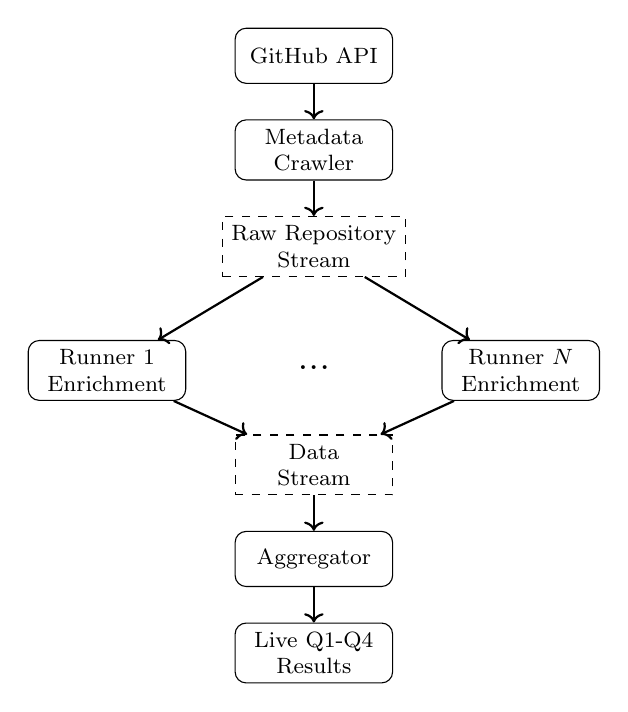
\begin{tikzpicture}[
    node distance=0.45cm,
    component/.style={
        rectangle,
        draw,
        rounded corners,
        align=center,
        minimum width=2.0cm,
        minimum height=0.7cm,
        font=\footnotesize
    },
    stream/.style={
        rectangle,
        draw,
        dashed,
        align=center,
        minimum width=2.0cm,
        minimum height=0.6cm,
        font=\footnotesize
    },
    arrow/.style={->, thick}
]

\node[component] (github) {GitHub API};
\node[component, below=of github] (crawler) {Metadata\\Crawler};
\node[stream, below=of crawler] (raw) {Raw Repository\\Stream};

\node[component, below left=0.8cm and 0.45cm of raw] (runner1) {Runner 1\\Enrichment};
\node[below=1.00cm of raw, font=\Large] (runnerdot) {...};
\node[component, below right=0.8cm and 0.45cm of raw] (runnern) {Runner $N$\\Enrichment};

\node[stream, below=2.0cm of raw] (processed) {Data\\Stream};
\node[component, below=of processed] (aggregator) {Aggregator};
\node[component, below=of aggregator] (results) {Live Q1-Q4\\Results};

\draw[arrow] (github) -- (crawler);
\draw[arrow] (crawler) -- (raw);
\draw[arrow] (raw) -- (runner1);
\draw[arrow] (raw) -- (runnern);
\draw[arrow] (runner1) -- (processed);
\draw[arrow] (runnern) -- (processed);
\draw[arrow] (processed) -- (aggregator);
\draw[arrow] (aggregator) -- (results);

\end{tikzpicture}
\caption{High-level architecture of the GitHub analytics system. The crawler
collects repository metadata, runners enrich the records using additional
GitHub API requests, and the aggregator continuously updates the analytics
results.}
\label{fig:architecture}
\end{figure}

\subsection{Deployment and Automation}
The system is intended to run across multiple cloud virtual machines using
containerized services. The master node will host the coordination services,
while the worker nodes will run the services responsible for data processing.
Docker is used to containerize each service, while Docker Swarm is used for
orchestrating these services across a cluster of one Manager and maximum four
Workers. This deployment model supports scalability experiments by allowing the
number of runners and the number of worker machines to be changed.

\subsection{Stream Processing with Apache Pulsar}
Apache Pulsar is used as the streaming layer between the crawler, runners, and
aggregator. The crawler acts as a producer, while the runners act as both
consumers and producers. Finally, the aggregator consumes from the runners. As a
result, the crawler does not need to know how many runners are active, and the
processing stage can be scaled independently. The streaming layer also helps
improve locality by distributing records to runners on worker nodes instead of
using a single centralized enrichment component. Each runner processes its
assigned records locally and publishes the data back to the stream. This reduces
unnecessary data movement while allowing more runners or worker machines to be
added without changing the crawler or aggregator.


\subsection{Data Collection}
The crawler is responsible for collecting repository metadata from the GitHub
API. Since the GitHub search interface limits the number of results returned by
a single query, the crawler divides the collection process into smaller queries
and uses pagination. Crawling can take a significant amount of time,
particularly for large datasets, and the GitHub API also imposes request limits.
Re-crawling data for days that have already been collected would therefore be an
inefficient use of resources. For this reason, collected results are cached on
disk for each day and reused across runs whenever data for that day is
needed again. The crawler also removes duplicate repositories before publishing
records to the stream. This ensures that each repository is processed only once
by the downstream stages.

The collected metadata provides the initial information needed by the pipeline.
Some analytics can be derived directly from this metadata, while others require
additional enrichment through the GitHub API. Therefore, the crawler only performs
the initial collection step, and the runners are responsible for gathering any
extra information needed by the later analytics stage.


\subsection{Enrichment and Aggregation}
The runners enrich repository records by retrieving the additional information
needed for the analytics questions. Commit activity is estimated by querying
the GitHub commits endpoint, while unit-test and CI/CD indicators are detected
by checking selected repository paths and configuration files. This avoids
downloading the full repository while still providing the extra information
needed for the analytics stage.

To reduce communication overhead, runners can send the data in batches of
configurable batch size. The aggregator consumes these data and re-evaluates the
current global answers to the four project questions. Since aggregation is
performed continuously, the system produces live results that are updated as
more repositories are processed.

\section{Experiments and Results}
\label{sec:experiments}

\subsection{Experimental Setup}
% Describe:
% - hardware / VM setup,
% - number of VMs,
% - Docker deployment,
% - dataset size,
% - number of runs,
% - metrics.
%
% Metrics can include:
% - total processing time,
% - throughput,
% - number of processed repositories,
% - speedup,
% - correctness of Q1--Q4 analytics.

\subsection{GitHub Analytics Results}
% Present the required analytics:
%
% Q1. Top 10 programming languages by number of repositories.
% Q2. Top 10 most frequently updated repositories.
% Q3. Top 10 programming languages with unit tests.
% Q4. Top 10 programming languages with both unit tests and CI.

%\begin{figure}[!t]
%    \centering
%    \includegraphics[width=\linewidth]{figures/top_languages.pdf}
%    \caption{Top 10 programming languages by number of repositories.}
%    \label{fig:top-languages}
%\end{figure}
%
%\begin{figure}[!t]
%    \centering
%    \includegraphics[width=\linewidth]{figures/top_commits.pdf}
%    \caption{Top 10 most frequently updated repositories.}
%    \label{fig:top-commits}
%\end{figure}
%
%\begin{figure}[!t]
%    \centering
%    \includegraphics[width=\linewidth]{figures/top_test_languages.pdf}
%    \caption{Top 10 programming languages by number of repositories with unit tests.}
%    \label{fig:top-tests}
%\end{figure}
%
%\begin{figure}[!t]
%    \centering
%    \includegraphics[width=\linewidth]{figures/top_test_ci_languages.pdf}
%    \caption{Top 10 programming languages by number of repositories with both unit tests and CI.}
%    \label{fig:top-tests-ci}
%\end{figure}

\subsection{Experiment 1}
\subsection{Experiment 2}
...
\subsection{Experiment ...}


\subsection{Discussion}
% Discuss:
% - what worked well,
% - what the main bottlenecks were,
% - whether scaling was close to linear,
% - whether partitioning helped,
% - limitations caused by GitHub API rate limits,
% - limitations of unit-test and CI detection heuristics.

\section{Conclusion}
\label{sec:conclusion}
% Summarize:
% - what system was built,
% - how Pulsar was used,
% - what experiments were performed,
% - what the main findings were,
% - possible future work.

% References
\bibliographystyle{IEEEtran}
\bibliography{main}

\end{document}
